% 
%% Copyright 2007, 2008, 2009 Elsevier Ltd
%% 
%% This file is part of the 'Elsarticle Bundle'.
%% ---------------------------------------------
%% 
%% It may be distributed under the conditions of the LaTeX Project Public
%% License, either version 1.2 of this license or (at your option) any
%% later version.  The latest version of this license is in
%%    http://www.latex-project.org/lppl.txt
%% and version 1.2 or later is part of all distributions of LaTeX
%% version 1999/12/01 or later.
%% 
%% The list of all files belonging to the 'Elsarticle Bundle' is
%% given in the file `manifest.txt'.
%% 

%% Template article for Elsevier's document class `elsarticle'
%% with numbered style bibliographic references
%% SP 2008/03/01

\documentclass[final,1p,times]{elsarticle}
\usepackage{amsmath,float,epsfig,subfigure, wrapfig}
\journal{Robotics and Autonomous Systems}


\begin{document}

\begin{frontmatter}

%\title{Enhancing the Stroke Palette for Robotic Drummers - A Physical Model Approach}

\title{A Generative Physical Model Approach for Enhancing the Stroke Palette for Robotic Drummers}

 \author[gt]{Deepak Gopinath\corref{cor1}}
 \ead{deepakedakkattilgopinath2015@u.northwestern.edu}
 
 \author[gt]{Gil Weinberg}
 \ead{gilw@gatech.edu}
 
 \cortext[cor1]{Corresponding author}
  
%  \address[nu]{Department of Mechanical Engineering, Northwestern University, Evanston, IL, 60208, USA}
%
%  \address[ric]{Rehabilitation Institute of Chicago, Chicago IL, 60611 USA}
   \address[gt]{Georgia Tech Center for Music Technology, Georgia Tech, Atlanta, GA, 30318, USA}

\begin{abstract}
	Achieving human-like musical expressivity in musical robots has been a long standing goal for roboticists and musicians who work in the emerging field of robotic musicianship. In robotic drumming, a major subfield of robotic musicianship, research towards achieving this goal has focused on the development of musical analysis and improvisational algorithms, design of robots that respond in a contextually appropriate way to music and methods to utilize gestures in collaborative music making. This research addresses the ``what" in robotic drumming, that is, what are the notes, dynamics, inter-onset times and the rhythmic parameters that a robot would play in response to the musical analysis. Much less research has gone into ``how" each of these notes are played and how to enrich the acoustical and timbral expression of robotic drummers.
	
	The main technical contribution of this work is a generative model for stroke generation in robotic drummers based on the physics of the interaction between human hand and a drumstick. A wide palette of strokes such as multiple bounce strokes, double, triple strokes can be generated using the same model by varying one single parameter, \textit{the time-varying torque applied by the thumb on the stick}. We have also developed a number of post processing tools to further modify the strokes produced by the physical model in an effort to simulate and capture the acoustic variety and richness of natural human drumming.
	We present results from a pilot study in which 22 subjects participated in a listening test in which they listened to 10 pairs of audio files, each consisting of a human and a robotic drummer playing multiple bounce strokes. Inferential confidence interval approach was used to determine the maximum probable difference between the data obtained from the listening test and a simulated experiment in which the robotic drummer was perceptually indistinguishable from a human drummer. The results indicates that this generative physics model marks an important step towards achieving human-like musical expressivity in robotic drummers.
%	 The evaluation results showed that the observed data was statistically equivalent to the subjects resorting to a blind guess in order to distinguish between a human playing a multiple bounce stroke and a robot playing a similar kind of stroke. A subjective evaluation was conducted and it was observed that, statistically, the subjects were unable to distinguish a multiple bounce stroke played by a human from a similar kind of stroke played by a robotic drummer. (edit) 
\end{abstract}
\begin{keyword}
	Robotic Musicianship, Musical Expressivity, Physical Modeling, Drumming
\end{keyword}
\end{frontmatter}
\section{Introduction}
The goal of this work is to enhance the stroke generation capabilities and
musical expressivity of robotic drummers. Expressivity can manifest itself
in many forms in drumming and music. Variations in timbre, stroke types
and activity rates (number of note events per unit time) all contribute to the meaning and expression of a musical strokes and
phrases. For human drummers, as they learn the language of the instrument
and the idiosyncrasies of musical styles, the rhythmic content of the music becomes only one aspect of music making. The question of ``how" to play each note becomes critical.

The focus of this research is to control the stick motion of robotic drummers thereby addressing the question of ``how" a stroke is executed. The approach here is to develop a generative model that captures the physics of a drum stroke (focusing on multiple bounce strokes) as performed by a human drummer from first principles and implement the model in a robotic drummer utilizing proper controller design. It has to be noted here that the goal of the model is not an exact replication of a multiple bounce stroke played by a human, but to create a similar kind of perceptual effect in the listener. 
%Furthermore, there is no one way to play a multiple bounce stroke and therefore establishing a ``ground" truth for objective evaluation is not sensible.

There are primarily two kinds of drum rudiments: rudiments that focus on controlling the exact number of bounces after the primary stroke (for example, single strokes, double strokes, triple strokes) and rudiments that control the statistical aspects of the stroke such as density of the bounces (closed roll)~\cite{rich2005buddy}. Non-standard bounce behavior (multiple bounce strokes in which the frequency of bounces change over time) is used for finer musical expressions and ornamentations in soloing and jazz accompaniment.

The former type can be implemented in a robotic drummer by specifying the number of ``single" hits that need to be concatenated to produce
the rudiment, whereas the latter can be achieved by using generative
models, such as the one developed in the present work. The entire process of embedding a robotic drummer with the capability to play single hits (or a combination of single hits) and multiple bounce strokes (with varying stroke profiles, loudness and duration) is equivalent to teaching a robotic drummer the building blocks of the drumming language.

The generative drumming model developed in the present work can also be used to produce atypical drumming behaviors in robotic drummers	by harnessing the speed and computational capabilities of a computer. For
example, a typical multiple bounce stroke by a human drummer has an exponentially decaying amplitude envelope (due to the effect of gravity). With the proposed model, it will be possible to model a system in which the gravity is changing over time, thereby create humanly impossible decay envelopes for the strokes. 

\section{Related Work}	
Several approaches have been adopted by researchers for the design of actuator mechanisms for robotic musicians. One of the most common actuator
mechanisms adopted is a motor/solenoid system that strikes the membrane
with a stick~\cite{kapur2007comparison}. In a solenoid system the force of the drum strike is proportional to the voltage that is applied to the solenoid. Typically in a MIDI triggered solenoid system, every drum strike corresponds to a single MIDI message\footnote{http://www.midi.org/aboutmidi/tut\_protocol.php}. Therefore, in a MIDI driven robotic drummer, a multiple bounce stroke can only be accomplished by sending a separate message for every individual hit in the stroke. However, humans execute a multiple bounce stroke by manipulating additional parameters such as the initial velocity and position of the stick and the grip pressure. Therefore, a solenoid-based system, which can only trigger discrete hit commands, cannot simulate the natural manner in which human drummers operate.

Several studies have looked closely at the mechanics of human drumming
from an engineering and bio-physical standpoint. Hajian et. al have studied the relationship between grasp force and the stick bounce and have implemented a mass-spring model which explains the dynamics of a double stroke drum roll in a simple, single joint robot which uses pneumatic actuators~\cite{hajian1997drum}.

Another approach is to model the bounce as a restoring force that acts
on the drumstick upon contact, usually as a compressed spring with a spring
constant that is extremely high compared to the stiffness of the human hand.
Berdahl et. al in their work on developing a physically intuitive haptic drumstick adopt this approach and consider a lumped mass spring damper model to model the effect of fingers~\cite{berdahl2007physically}. However, the physical modeling approaches adopted by Hajian and Berdahl is
limited in their scope as only one category of drum stroke (a closed double stroke roll) is considered, the work cannot be generalized to produce other kinds of strokes.

Kim et. al have also modeled the dynamics of the interaction between the drumstick, drumhead and the fingers as a coupled mass-spring damper model and have used a variable stiffness actuator to realize the drum strokes in a robotic drummer~\cite{kim2014drum}. Different ranges of stiffnesses that correspond to single and double strokes have also been identified. However, Kim's work does not deal with multiple bounce strokes. Furthermore, the dynamic level of the second hit in the double stroke is much lower than the first hit, which is very different from how a human will play a double stroke. Moreover, it will be hard to use the model presented in~\cite{kim2014drum} to generate multiple bounce strokes. The work presented in this paper, do not suffer from such limitations as the force exerted by the finger on the stick can be modulated in such a way that the amplitude of hits remain consistent. 	

Another study undertaken by Andreas Wagner analyzed the interaction between the human hand, drum stick and the membrane, but no attempt was made to replicate the behavior in any kind of robotic percussionist~\cite{wagner2006analysis}. Wagner comes to the conclusion that the dominant factors that shape the interaction process between a drumstick and the drumhead are the deflection and the tension of the drumhead and the vibration of the drumstick. According to Wagner, the role of the human drummer is to determine the initial onset energy (which will determine the dynamic level) and the placement of the stroke (which will determine the modes excited in the drum). The influence of changing the grip of the stick is not considered in Wagner's work and is left for future research.

Weinberg and Driscoll attempted to expand the timbral possibilities of
a robotic drummer in their design of \textit{Haile}, a two armed robotic percussionist designed to play a native American drum~\cite{weinberg2006robot}. \textit{Haile} adopted a quasi-anthropomorphic design and utilizes two percussive arms that can move to different locations on the drum~\cite{weinberg2005haile, weinberg2006toward}. Weinberg's research also focuses on the perceptual, cognitive and algorithmic aspect of robotic musicianship and machine listening. Enhancing musical expressivity is achieved by improving the musical content, that is, produce rhythmic responses by using perceptually salient machine listening, improvisation algorithms~\cite{weinberg2007real, weinberg2006jam} and style modeling~\cite{nikolaidis2010playing}. Weinberg et. al also studied the importance of gestures and visual cues in improvised music and implement the same in robotic musicians~\cite{weinberg2007real, weinberg2009interactive}.

Concepts from physics have been successfully utilized for creating drumming systems, for example, in~\cite{degallier2006movement} a dynamical systems approach was adopted for online generation of drumming like motions for humanoid robots. The system was also able to switch between discrete (which will allow for isolated hits) and rhythmic modes and was able to generate trajectories for an arbitrary drum score. However, subjective evaluation was not performed with the system. 
Researchers of the Humanoid Robotics Group at MIT developed \textit{Cog} which could perform a wide variety of rhythmic as well as discrete tasks. Williamson et. al designed a compliant robot arm with six degrees of freedom and uses simple non-linear oscillators to control the arm~\cite{brooks1999cog}. The arms use series elastic actuators which incorporate physical springs at each joint. The main difference between traditional robot control and Williamson's approach is the way in which robot dynamics play a crucial role in the execution of the task. Williamson acknowledges that the traditional approach is more general and the non-linear oscillators are limited to those trajectories that are generated by the oscillators.

\section{Generative Physical Model for Stroke Generation}
Building on previous works, the present project aims to create a robotic
percussionist that can generate a variety of stroke types (single, double, multiple bounces), by controlling the time-varying torque provided by the thumb as a tunable parameter in a physical model. That is, this project addresses one of the most fundamental aspect of drumming, which is the ability for a drummer to hit a drum in diverse ways.
\subsection{Robotic Platform}

The robotic platform used in the present work is the \textbf{Robotic Drumming Prosthesis (RDP)} developed by the \textit{Robotics Musicianship Group} at \textit{Georgia Tech Center for Music Technology} in collaboration with \textit{Meka Robotics} for Atlanta based amputee drummer Jason Barnes. The PI controller used for position tracking is implemented in \textit{MATLAB/Simulink}\footnote{http://www.mathworks.com/products/matlab, http://www.mathworks.com/products/simulink} on a host computer running Ubuntu 14.04. High precision motor control is facilitated by using high resolution optical encoders mounted to the rear of the motors. The main microprocessor boards used in the device are proprietary boards from \textit{Meka Robotics} and are mounted directly in the main structure. The communication between the host computer and the board is over a high speed \textit{EtherCat} based control bus. 
\begin{figure}[h]
	\begin{center}
		\includegraphics[width = 1\hsize]{./figures/Fig1.pdf}
		%		\vspace{-2.5cm}
		\caption{Stick in rotational equilibrium}
		\label{HS}
	\end{center}
\end{figure}
\subsection{Simplified Model of Drumming Mechanics}

This work focuses on modeling the palm and finger
control while disregarding potential degrees of freedom at the elbow and the wrist. This is justified because the variations in multiple bounce strokes are typically brought about by using smaller muscle groups present in the fingers and wrist. 

The drumstick is treated as a uniform rigid rod rotating about a fixed pivot point. When the stick is in rotational equilibrium about the fulcrum, the torque due to gravity is balanced by a counter torque provided by the backside of the thumb (Figure~\ref{HS}). In order to produce a buzz stroke (a multiple bounce stroke), drummers typically release the stick by opening up the thumb letting the stick drop. Gravity will make the stick accelerate towards the drum head. Upon hitting the head, the thumb (and/or the fingers) is used to provide a time varying torque to control the after bounce profile (or restrict the motion of the stick).

This simple time varying torque model provides a physics framework
which can be used for generating different kinds of multiple bounce strokes. Based on the general shape of the torque profiles, a few stroke categories have been identified:
\begin{itemize}
	\item No External Torque (Only Gravity) --- In which there is no torque due to the thumb and the bounce behavior is similar to that of a bouncing ball.
	\item Constant External Torque --- In which the behavior is similar to that of a bouncing ball, but as if in an environment with stronger gravitational force. 
	\item Low to High variation in torque --- In which the initial onsets are widely spaced with a sudden increase in the frequency of onsets. 
	\item High to Low variation in torque --- In which the initial onsets are closer together followed by a sudden decrease in the frequency of onsets.
	\item Un-natural variations in torque --- In which the profiles are extremely hard to produce by human drummers, but can be possible in a physics simulation, thereby giving rise to strokes that can go beyond human capabilities.
\end{itemize}

\subsection{Derivation of the Dynamical Equation}
In Figure~\ref{TD}, let $L$ be the length of the drumstick, $x$ be the distance of the fulcrum from the tip and $m$ be the mass of the drumstick. $\theta$ is the angular displacement of the stick and $\theta = 0$ when the stick is parallel to the drumhead. As the stick moves downwards towards the drum, $\theta$ decreases (downward direction is taken as negative). The moment of inertia $I$ is given by
\begin{equation} \label{eq1}
I = \frac{m}{3L}(x^3 - (x-L)^3) = \frac{m}{3}(3x^2 - 3xL + L^2)
\end{equation}

The drum stick is treated as a freely rotating rod about a pivot point
which is at a distance of $x$ from the tip of the stick. Gravity acts at the center of mass which is approximately located at the midpoint of the stick and is at a distance of $k$ from the fulcrum. The thumb is in contact with the stick at a distance of $k'$ from the fulcrum.

The total torque($\tau_{total}$) acting on the drumstick can be written as
\begin{equation*} 
\tau_{total} = \tau_{gravity} + \tau_{ext}(t)
\end{equation*}
where $\tau_{gravity}$ is the torque due to gravity and the external torque $\tau_{ext}$ is a function of time $t$ and can have different kinds of profiles. 
Furthermore, 

\begin{figure}
	\begin{center}
		\includegraphics[width = 1\hsize]{./figures/Fig2.pdf}
		\vspace{-2.5cm}
		\caption{Detailed torque diagram}
		\label{TD}
	\end{center}
\end{figure}
\begin{gather*}
 \tau_{gravity} = -mgcos(\theta)k \\
 \tau_{ext}(t) = -F_{ext}(t)cos(\theta)k'
\end{gather*}
where, $F_{ext}(t) = ma_{ext}(t)$ and $a_{ext}(t)$ is the linear acceleration provided by the thumb. From Newton's laws we have 
\begin{equation*}
\tau_{total} = I\ddot{\theta}
\end{equation*}
where $\ddot{\theta}$ is the angular acceleration of the stick. 
Then,
\begin{equation} \label{eq2}
I\ddot{\theta} = \tau_{gravity} + \tau_{ext}(t) \\
\end{equation}
%\vspace{-0.7cm}
\begin{equation} \label{eq3}
I\ddot{\theta} = -mgcos(\theta)k  - ma_{ext}(t)cos(\theta)k'
\end{equation}
Substituting Equation~\ref{eq1} in Equation~\ref{eq3} and rearranging the terms we get
\begin{equation} \label{eq4}
\ddot{\theta} = -\frac{3cos(\theta)(gk + a_{ext}(t)k')}{3x^2 - 3xL + L^2}
\end{equation}

Since the geometrical relationship between the pivot point, the stick and
the drumhead is fixed, the vertical distance of the pivot point from the drumhead ($h$) is constant. From $h$ and $x$, the maximum angular displacement possible for the stick from steady state position can be calculated as
\begin{equation}
\theta_{max} = -sin^{-1}\left(\frac{h}{x}\right)
\end{equation}
In order to incorporate collisions of the stick with the drum, two approaches can be adopted. 

In the first approach, the forces acting upon the
stick at the moment of contact can be approximated and for a short duration the dynamical equation can be modified. In a more simplistic approach, the effect of all the contact forces is summarized and is treated as an inelastic collision. The collision is inelastic because there is a loss of energy due to the damping of the drumhead, sound produced, air resistance \textit{et cetera}. 
Therefore, when $\theta = \theta_{max}$ (condition for stick colliding with the drumhead), the velocity undergoes an instantaneous change in direction and magnitude given by,
\begin{equation}\label{eq6}
\dot{\theta}_{after} = -c\dot{\theta}_{before}
\end{equation} 
where $c$ is the coefficient of restitution (COR) between the drum stick and the drum head. The parameter $c$ can be computed explicitly if the mass of the drum stick, damping and spring constants of the drum head are known as in~\cite{berdahl2007physically}. A simpler approach, the one adopted in this work, is to experimentally determine the coefficient of restitution. If we model the drum stick as a bouncing ball falling freely under the influence of gravity, then the coefficient of restitution (COR) can be computed by comparing the maximum height the stick reaches after the first bounce to the height at which it was initially released (neglecting friction at the fulcrum and air resistance). Typically, for taut drum heads this value can be fairly high, whereas for low pitched drums, the value can be low. Futhermore, for the purposes of simulation this can be treated as a tunable parameter. 

The stick used for the study was a \textit{Zildjian Maple Mini-ball}\footnote{http://zildjian.com/Products/Drumsticks-and-Mallets/Maple-Series/Maple-Mini-Ball}. For this stick, the approximate values of all the variables involved are presented in Table~\ref{table:Table1}.
\begin{table}
	\caption{Parameters values for Zildjian Maple Miniball stick}
	\vspace{0.3cm}
	\centering
	\begin{tabular}{c c}
		\hline\hline
		\textbf{Parameter} & \textbf{Value}\\
		\hline
		$L$ & $0.39\;$m\\
		\hline
		$x$ & $0.27\;$m\\
		\hline
		$k$ & $0.075\;$m\\
		\hline
		$k'$ & $0.01\;$m\\
		\hline
		$h$ & $0.07\;$m \\ 
		\hline
		$\theta_{max}$ & $-0.2623\;rad$\\
		\hline
		$vol$ & $6.23\times10^{-5}\;$m$^3$\\
		\hline
		$\rho$ & $600\;$kg/m$^3$\\
		\hline
		$m$ & $0.0373\;$kg\\
		\hline
		
	\end{tabular}
	\label{table:Table1}
\end{table}
Substituting the parameter values from Table~\ref{table:Table1} in Equation~\ref{eq4} with acceleration due to gravity $g = 9.8\;$m/s$^2$ we have,
\begin{equation} \label{eq7}
\ddot{\theta} = -\frac{cos(\theta)\times(0.735+(0.01\times a_{ext}(t)))}{0.0714}
\end{equation}

This is a second order differential equation (with $a_{ext}(t)$ as the time varying input to the system) that can be solved using standard numerical methods. The external linear acceleration $a_{ext}(t)$ is in the range $0\;$--$\;250\;$m/s$^2$. For a stick with $m = 0.0373\;$kg this corresponds to a linear force of approximately in the range of $0\;$--$\;10\;$N. This is the characteristic force range that fingers can produce during the interaction with a drumstick while performing a drum stroke~\cite{hajian1997characterization}. 
\begin{figure}[H]
	\begin{center}
		\includegraphics[width = 1.02\hsize]{./figures/Fig3.pdf}
		\caption{Implementation Framework}
		\label{FW}
	\end{center}
\end{figure}
\subsection{Implementation of Stroke Profiles in the RDP}
The generative physical model described in the previous subsection provides motor angle trajectories for different kinds of multiple bounce strokes. Once the stroke profiles are generated, a successful implementation of the same in the RDP requires proper controller design and tuning. The RDP uses a PI controller to do reference trajectory tracking. 

For the purposes of this work, the physical model was implemented in \textit{MATLAB/Simulink}. Various multiple bounce stroke profiles were simulated from the physical model and the results were compiled into a library of stroke profiles. These stroke profiles were then stored as text files in the host computer which communicates with the RDP. At runtime, these stroke files were loaded into memory and then accessed depending on the musical application. Musical compositions and patterns (which are specified as how the motor angle changes with time) were generated using custom C++ code which utilized the stroke profiles as fundamental musical building blocks. 17 different strokes were created for the stroke library. Our system implementation is overviewed in Figure~\ref{FW}.

The success of a PI controller in tracking a given reference trajectory (minimum error
between actual trajectory and the reference) depends on how well the controller gains have been tuned. Formal methods of tuning the controller gains were not adopted in this work, instead
the exact values of the gains were determined manually by trial and error. Since the diversity of simulated strokes was very high, we recognized that one particular combination of controller gains would not necessarily guarantee robust reference tracking for different kinds of strokes. However, a trade-off was made and the controller gains were fixed for all the stroke profiles. 
%\vspace{-3cm}

\subsection{Creativity in Model Parameter Tuning}
Regardless of the exact values of the model parameters, the goal
of this work is to obtain a angular position vs. time profile that can be given as a reference trajectory to the PI controller. For multiple bounce strokes there is no one ``correct'' way of playing a stroke. By changing the input acceleration profiles in a continuous manner, infinitely many stroke profiles are possible. The engineer/designer of the system can be more creative and set the model parameters to non-standard values to generate un-natural stroke profiles, which will then enhance the stroke palette that a composer has at his/her own disposal. Furthermore, the stroke profiles may also be post processed to create artificial variations. Although the variations might never be possible in a natural way, the musical relevance and utility justifies this approach. Some of the possible post processing operations that can be applied on the stroke profiles are time stretching, compression (changes the dynamic level) and time reversal. A more detailed explanation of the musical applications of the work can be found in~\cite{edakkattil2015enhancing}.

\section{Simulation Results}
This section presents the results of simulations for different time varying
external force profiles. Four different profiles are presented.
The physical model given by Equation~\ref{eq7} along with the collision condition given by Equation~\ref{eq6} is simulated for time $t \in [0,5]$ in \textit{MATLAB/Simulink}.
 For all the simulations $\theta_{init} = 0$, $\theta_{max} = -0.2623\;$rad, $\dot{\theta}_{init} = 0$,  $g = 9.8\;$m/s$^2$ and COR$\;=0.86$.
%In each one of the figures, the top sub-plot shows the angular position of
%the stick (in radians) vs. time profile, and the bottom sub-plot shows the time
%varying linear acceleration provided by the thumb. Time is on the x-axis.

Figure~\ref{NF} shows the simulation result in the case where the stick is allowed to bounce freely on the drum head. The result is very similar to that of a bouncing ball. In drumming, this can be achieved by balancing the stick at the first joint of the forefinger and then letting it go and having the thumb not to be in contact with the stick at all times. This particular stroke is usually employed in a more improvisational musical context which calls for more \textit{rubato} playing. By changing the initial angle and the velocity a large number of variations can be achieved.

Figure~\ref{LH} shows the simulation result in the case where the grip force on the stick starts off as a low value and then increases suddenly and drops back to a smaller value. The effect of increasing
\begin{figure}[H]
	\begin{center}
		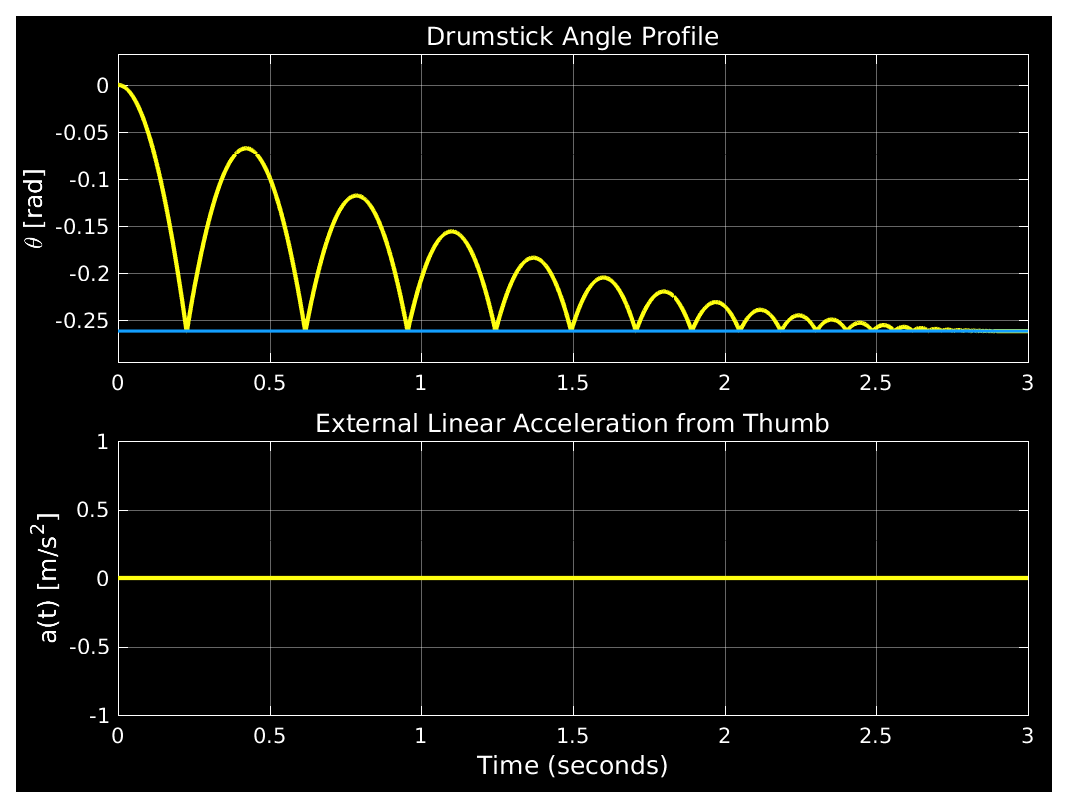
\includegraphics[scale =0.65]{./figures/Fig4.eps}
		\caption{No external force from thumb - Free bounce}
		\label{NF}
	\end{center}
\end{figure}
\begin{figure}[H]
	\begin{center}
		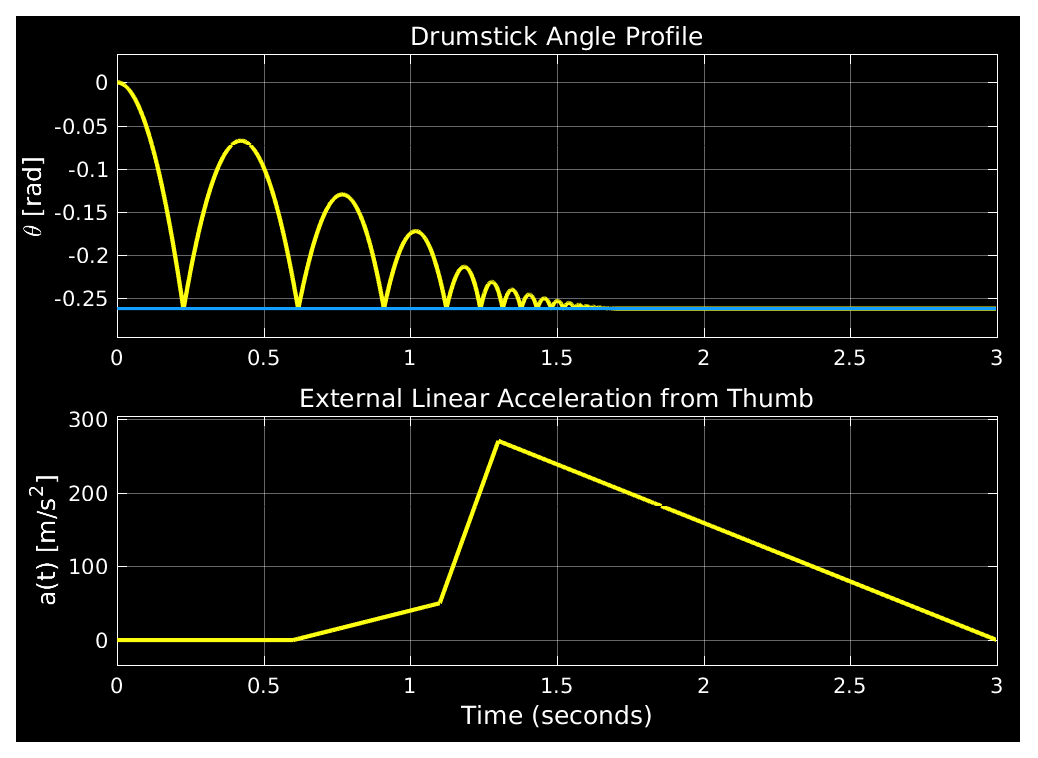
\includegraphics[scale =0.67]{./figures/Fig5.eps}
		\caption{Low grip force to high grip force}
		\label{LH}
	\end{center}
\end{figure}
\noindent the force is to increase the frequency of bounces drastically (between 1s and 2s in the plot). Once the stick comes to rest on the surface of the drum, further changes in the external force do not have any effect on the position of the stick as this would only result in further pressing down the stick into the drum. This kind of stroke can be employed in a variety of musical situations ranging from free improvisation, jazz accompaniment and classical snare drum playing.
\begin{figure}[H]
	\begin{center}
		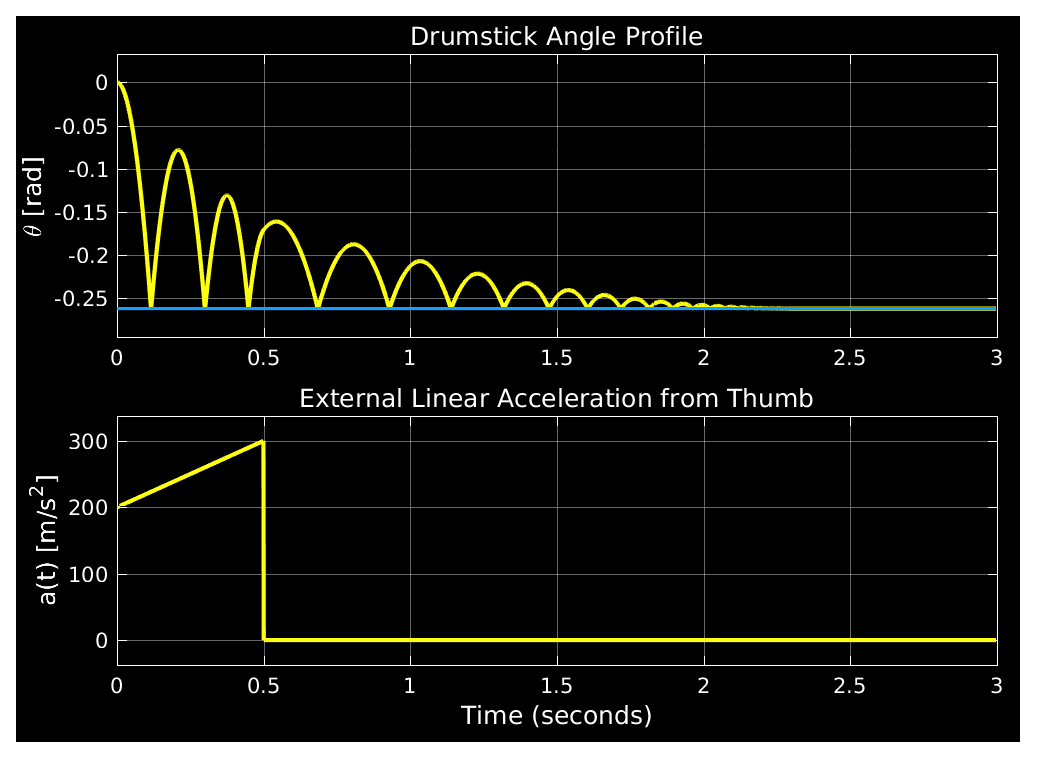
\includegraphics[scale =0.67]{./figures/Fig6.eps}
		\caption{High grip force to low grip force}
		\label{HL}
	\end{center}
\end{figure}


Figure~\ref{HL} shows the simulation result in the case where the grip force on the stick starts off at a high value and decreases suddenly to zero. The effect of this profile is that the initial few bounces happen at a relatively higher frequency followed by a sudden reduction in the rate of bounces, as can be seen in the plot after 0.5s. Once the external force becomes zero, the only force acting on the stick is gravity and the position profile is same as that of a free fall. This is a slightly unnatural multiple stroke which calls for a higher skill level from the drummer, although the effect can be very interesting musically, especially in a rubato/free improvisational context

The generality of the model is demonstrated in the simulation result shown in Figure~\ref{SB}.
In drumming, fingers are often used to generate fast pulsing actions so that a multiple
bounce stroke can be continued and sustained for a longer duration. The constant pulses
from the fingers add more energy into the system and compensates for the energy lost due
to the inelastic collision. The phase and amplitude of the pulses becomes very critical and in the case of human drumming, the constant feedback loop (haptic and aural) helps in providing the pulses at the right time. Typically, this leads to a resonant frequency in which the long term behavior becomes constant. In Figure~\ref{SB}, the impulses from the fingers are approximated by using a square wave with a duty cycle of $5$\%, period length = $0.4$s and amplitude = $189\;$m/s$^2$.

This indicates that the generative model can have wider applicability than just to generated multiple bounce strokes and that any kind of stroke may be produced by providing the appropriate kind of thumb force profile.
\begin{figure}[H]
	\begin{center}
		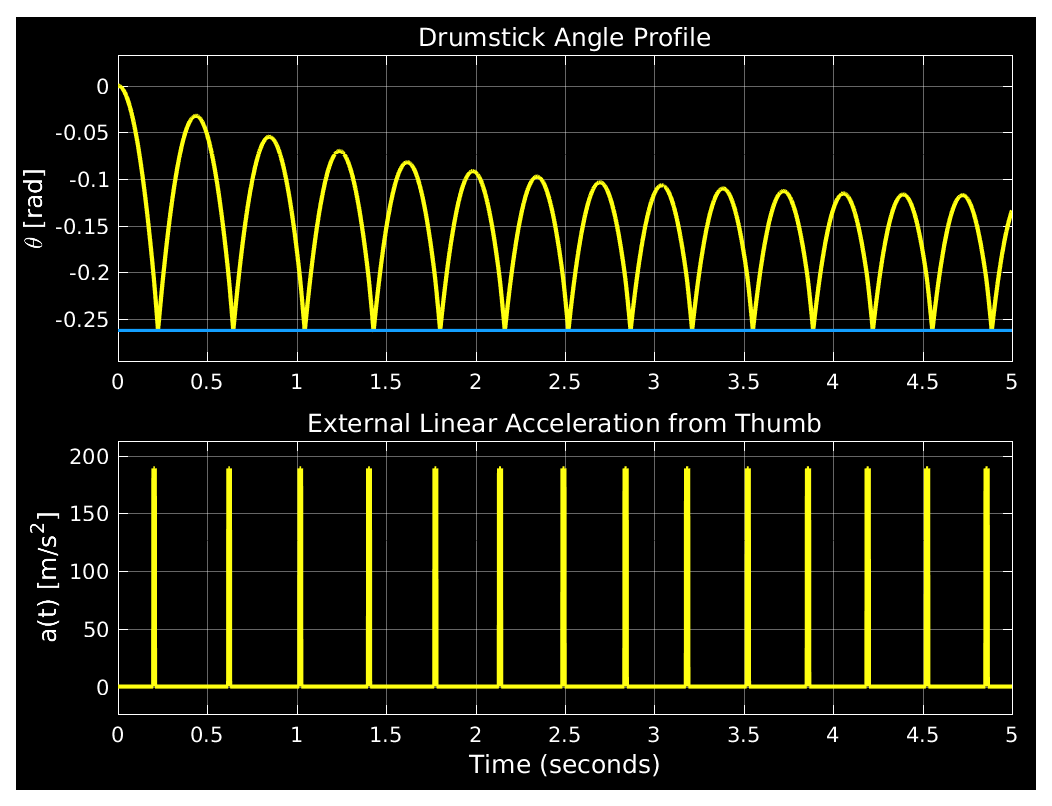
\includegraphics[scale =0.67]{./figures/Fig7.eps}
		\caption{Sustained bounce due to regular finger pulses.}
		\label{SB}
	\end{center}
\end{figure}
\section{Evaluation and Results}
We performed a subjective evaluation of our physical model and its implementation using a listening test in which participants were asked to distinguish between and rate the similarities between the audio recordings of a human and a robotic drummer performing multiple bounce strokes of the same type. Objective evaluation for this work was ruled out because establishing a ground truth is meaningless as there is no singular way to play a multiple bounce stroke. As stated in the introduction, the goal is to achieve perceptual similarity, therefore a subjective test was chosen. 

\subsection{Methodology}
Twenty two subjects (17 males, 5 females) were recruited for the study.
All subjects have had previous musical experience.

The subjects participated in a short listening test in which they listened
(via headphones) to 10 pairs of audio files (volume normalized), lasting 2-3s each. Each audio pair consisted of a human drummer playing a multiple
bounce stroke of two different types (``Only Gravity" and ``Low to High") on a snare drum (either with the snares on or with the snares off) and the robotic drummer playing the same type of multiple bounce stroke generated by our model in a random order. Different areas on the drumhead were used for playing the stroke in order to randomize the timbral quality of the audio recordings.

After listening to each pair of audio files, the subjects were also asked to answer the following three questions
\begin{itemize}
	\item Which one of the audio files is played by human and which one is played by a robot?
	\item On a scale of 1-5, how sure were you about the answer to the previous question?
	\item On a scale of 1-5, rate the similarity of the two audio files with respect to the approximate number of bounces and how the volume of each stroke fades out? Please try to ignore the timbre when you do the similarity judgment.
\end{itemize}

\subsection{Analysis and Results}
For the purposes of analysis we consider two groups of data. The first group (Group A) consists of the responses obtained from the listening test and is denoted by \{$p_i$\} such that $i \in [1,22]$  (number of subjects) and $p_i \in [0,10]$ (number of incorrect responses per subject).
%The mean number of incorrect answers across all subjects and all audio pairs was found to be $4.227$, while the standard deviation was $2.654$.
% However, we are interested in distribution of the mean itself. That is, if we were to repeat the experiments on different 22 subjects many times how will the distribution of the mean number of incorrect answers look like. In order to generate this distribution we employ the technique of \textit{empirical bootstrapping}. 

For the second group (Group B) we consider an alternate hypothetical scenario in which a multiple bounce stroke from the generative model is \textit{perceptually indistinguishable} from a multiple bounce stroke played by a human. During the listening test with Group B, to maximize the chances of answering correctly, the best option for a listener is a $50$-$50$ guess. It is very likely that in such a experiment the mean number of incorrect answers will be close to $5$ as well. Furthermore, it is easy to have a computer simulation of this scenario. 

Group B consists of simulated data and is denoted by \{$q_i$\} such that $i \in [1,22]$ (number of subjects) and $q_i \in [0,10]$) (number of incorrect responses per subject). 
Simulations were done in \textit{MATLAB} and the descriptive statistics from both Group A and Group B are presented in Table~\ref{table:Table2}. Note that for Group B the descriptive statistics were computed by averaging over multiple simulation runs. 
%\vspace{-0.5cm}
\begin{table}[h!]
	\centering
	\caption{Descriptive statistics for Group A and B}
	\vspace{0.2cm}
	\begin{tabular}{||c c c||} 
		\hline
		Statistic & Group A & Group B \\  
		          & ($p_i$) & ($q_i$) \\ [0.5ex]
		\hline\hline
		Mean & 4.227 & 4.999 \\ 
		SD & 2.654 & 1.564 \\
		N & 22 & 22  \\
		SE & 0.566 & 0.336 \\ 
		Lower 95$\%$ CI & 3.051 & 4.3\\ 
		Higher 95$\%$ CI & 5.404 & 5.698 \\ [1ex]
		\hline
	\end{tabular}
	\label{table:Table2}
\end{table}
%Once we have the bootstrapped distribution (Group I) and computer simulated distribution (Group II), the question then is: \textit{how closely does the perceptual effect created by the multiple bounce stroke generated using the physics model resemble the ones by a multiple bounce stroke played by a human?}. This can be then thought of a test for statistical equivalence between the two groups. The question of how successful the generative model

The effectiveness of the physical model in generating multiple bounce strokes that are perceptually similar to the ones played by humans can then be quantified by computing the \textit{maximum probable difference} between the means of Group A and Group B. This can be computed using the \textit{inferential confidence interval} (ICI) approach as described in~\cite{tryon2001evaluating,tryon2008inferential}.
%The success of the generative physics model can then be evaluated by performing a statistical equivalence test between Group A and Group B. Statistical equivalence test was performed using \textit{inferential confidence approach} as described in~\cite{tryon2001evaluating,tryon2008inferential}. 
In Tryon's approach the scaling factor $E$ (for $N_p$ = $N_q$) which will determine the extent to which the descriptive confidence interval must be reduced to obtain an inferential confidence interval is computed using
\begin{equation}
E = \left(\frac{\sqrt{S_{\overline{p}}^{2} + S_{\overline{q}}^{2}}}{S_{\overline{p}} + S_{\overline{q}}}\right).\left(\frac{t_{pq}^{\alpha/2}}{t_{p}^{\alpha/2}}\right)
\end{equation}
where $S_{\overline{p}}$ and $S_{\overline{q}}$ are the standard errors for Group A and Group B respectively, $t_{pq}^{\alpha/2}$ is the t-value at $\alpha$ significance level for the difference between the two means and $t_{p}^{\alpha/2}$ ($= t_{q}^{\alpha/2}$ since $N_p$ = $N_q$) is the t-value for each group. 
The maximum probable difference ($Rg$) between the means of the two groups is then computed as 
\begin{equation}
Rg = (m_q - m_p) + t_{p}^{\alpha/2}E(S_{\overline{p}} + S_{\overline{y}}) 
\end{equation}
where $m_p$ and $m_q$ are the means of Group A and Group B respectively.
For $\alpha=0.05$ and $N_p = N_q = 22$, $\;t_{pq}^{\alpha/2} = 2.0181$ and $t_{p}^{\alpha/2} = t_{q}^{\alpha/2} = 2.0796$.

%The ICI approach also requires the specification of $\Delta$ (the maximum difference that is unimportant or can be dismissed on substantive grounds), such that when $Rg < \Delta$ statistical equivalence can be claimed. 

%The choice of $\Delta$ is usually based on theoretical considerations, however, for the present work, this is really hard to determine and can be any arbitrary value (elaborate ,maybe examples from drug industry as to how delta values are specified?). Here, we choose $\Delta$ in the range of $10-15\%$. We can claim that Group A and Group B are statistically equivalent or in other words that multiple bounce strokes produced by the physics model are perceptually indistinguishable from multiple bounce strokes played by humans if $Rg < 10-15\%$. 

With the values in Table~\ref{table:Table2}, $Rg$ for Group A and Group B was computed to be $20.99\%$. 

The ICI approach also can be used to determine statistical equivalence between the two groups, however this requires the specification of the quantity $\Delta$ which is the \textit{maximum difference that is unimportant or can be dismissed on substantive grounds}. However, the choice of $\Delta$ is domain specific and based on theoretical considerations. In the present context this is not well defined and an arbitrary choice of $\Delta$ will be meaningless. A smaller value of $Rg$ implies that it will be a stronger case for statistical equivalence as the $\Delta$ can also be made smaller. 

Furthermore, no correlations were found between
the number of incorrect answers and how sure the subjects were when they
answered the first question. Similarly, no correlations were found between
the similarity ratings and the number of incorrect answers. 
\section{Discussion}

Maximum difference between the two group means occurs when the mean of Group A is placed against the bottom of its inferential CI and the mean of Group B is against the top of its inferential CI (assuming $m_p < m_q$). This represents the worst case scenario. 

We think that  a maximum probable difference of $20.99\%$ can further be improved by better hardware and controller design.
%The PI controller in this system is used to do reference trajectory tracking and the reference is obtained from the physics model.
 The tail end of the reference trajectory obtained from the model usually consists of high frequency bounces and the PI controller is not robust enough to keep up with the higher bandwidth signal. As a result, especially for strokes belonging to ``Only Gravity" category played by the robotic drummer, the tails will become shorter than when played by human drummers. This will create a significant perceptual difference which is easily identifiable. 

Furthermore, only linear piecewise force profiles were used for generating the stroke profiles. However, for a human drummer the force profile produced by the thumb is likely to be more complex. High quality force sensors attached to the stick can probably be used to determine the exact time-varying force profile produced by the thumb when a human plays and this data can then be used as the input to the physical model to generate reference trajectories. This might result in more accurate replication of human-like strokes (although exact mimicry of a human stroke is not the goal) and help in reducing the maximum probable difference. 

We also recognized
that although we explicitly asked subjects to ignore the timbral differences
between the audio files, subjects might not have been able to ignore such
differences as the human auditory system is very sensitive to timbral changes.
Even though the number of bounces and the volume decay envelope were
similar to that of a human stroke, the timbral differences might have been
fairly prominent and could have influenced the subjects' judgment.
%Why is there such a difference? Issue with not having a robust controller. PI control is not able to keep with high bandwidth reference trajectories And therefore the tail can be shorter for (no gravity case). The force profiles considered are only linear piecewise functions. This may be a limitation. NEed to look into FSR data and analyse how 

\section{Conclusions}
The main contribution of this work is the development of a generalized physical model for drum stroke generation aimed at expanding the stroke palette for robotic drummers. This marks an important step towards achieving human-like musical expressivity in robotic drummers. The system that is presented is agnostic to the exact specifications of the robotic drummer, due to the complete decoupling of the stroke generating mechanism and the controller in the robotic drummer. 
The model developed in this work was implemented on the \textit{Robotic Drumming Prosthesis} and a PI controller was used to perform trajectory tracking. The evaluation of the model was done by employing a listening test in which subjects listened to 10 pairs of audio files, each consisting of a human and a robotic drummer playing multiple bounce strokes. Inferential confidence interval approach was used to determine the maximum probable difference between the data obtained from the listening test and a simulated experiment in which the robotic drummer was perceptually indistinguishable from a human drummer. The maximum probable difference was computed to be $20.99\%$. The project has also shed light on the generative mechanisms that play an important role in creating diversity in the drum strokes produced by a human drummer and opening the doors for future experimentations in developing novel artificial drum strokes that might be beyond human capabilities.
\section*{Acknowledgments}
This work was supported by National Science Foundation (NSF) (Grant No: 4866604). We also would like to thank Prof. Alexander Lerch for valuable suggestions and advice during the early stages of this work and Dr. Vishnu Sreekumar for clarifications regarding the statistical analysis during the revisions. 
\section*{References}
\bibliographystyle{elsarticle-num} 
\bibliography{ras_deepak_gil_bib}
\section*{Vitae}
\begin{wrapfigure}[12]{R}{0.4\textwidth}
	\begin{center}
		\vspace{-.6cm}
		\includegraphics[width=0.25\textwidth]{./figures/deg.jpg}
	\end{center}
%	\vspace{-.45cm}
	\label{PAF}
\end{wrapfigure}

\noindent Deepak E. Gopinath is a first-year doctoral student in the Mechanical Engineering Department at Northwestern University and works with Dr. Brenna Argall in the Assistive and Rehabilitation Robotics Laboratory at the Rehabilitation Institute of Chicago. He completed his B.Tech in Engineering Physics from IIT Bombay in
2003, after which he moved to Boston, USA to pursue a Professional Diploma in Music, at Berklee College of Music majoring in Composition and Jazz Performance. Prior to coming to Northwestern, he pursued a Master's in Music Technology at Georgia Tech under Dr. Gil Weinberg where he worked in the field of Robotic Musicianship. His current interests are in assistive robotic manipulation and developing mathematical formalisms for shared control architectures in assistive robotics. \\ 
\begin{wrapfigure}[12]{R}{0.4\textwidth}
	\begin{center}
		\vspace{-.7cm}
		\includegraphics[width=0.24\textwidth]{./figures/gilw.jpg}
	\end{center}
	\vspace{-.45cm}
\end{wrapfigure}

\noindent Gil Weinberg is the founding director of the Georgia Tech Center for Music Technology. He is a professor in the School of Music and an adjunct professor in the School of Interactive Computing. Weinberg's research aims at expanding musical expression, creativity, and learning through meaningful applications of technology. His research interests include robotic musicianship, new instruments for musical expression, mobile music, and sonification. Weinberg received his M.S. and Ph.D. degrees in Media Arts and Sciences from MIT and his B.A degree from the Interdisciplinary Program for Fostering Excellence in Tel Aviv University.
\end{document}
\end{table}
